\subsubsection{FOC-Treiber}
\label{subsubsec:Inbetriebnahme_FOC_Treiber}
Der FOC-Treiber wird mit einem Testprogramm in Betrieb genommen. Das Programm initialisiert die benötigte Hardware des Mikrocontrollers (UART, SPI, Pins), enthält die Library des FOC-Treibers und ermöglicht das Debugen über die serielle Schnittstelle. Die Software TMCL-IDE hilft bei der Bestimmung der Parameter für den FOC-Treiber. Welche Register wie beschrieben sind ist im Anhang Kapitel \ref{Appendix:TMC4671_Register} zu sehen. Die Initialisierung sowie das Auslesen gewisser Register ist mit der Testapplikation ''\textit{3\underline{ }Motor\underline{ }Openloop}'' möglich. Sie ist im Softwareordner auf dem USB-Stick oder auf Github \cite{aebi_projekt-6softwareatmega_2020} zu finden.

Es wird erwartet, dass der FOC-Treiber die Gate-CTRL-Signale erzeugt. Der Duty-Cycle muss sich ändern, sobald der FOC-Treiber die Open-Loop-Drehung startet.

\paragraph{Setup}\mbox{}

\begin{figure}[H]
	\centering
	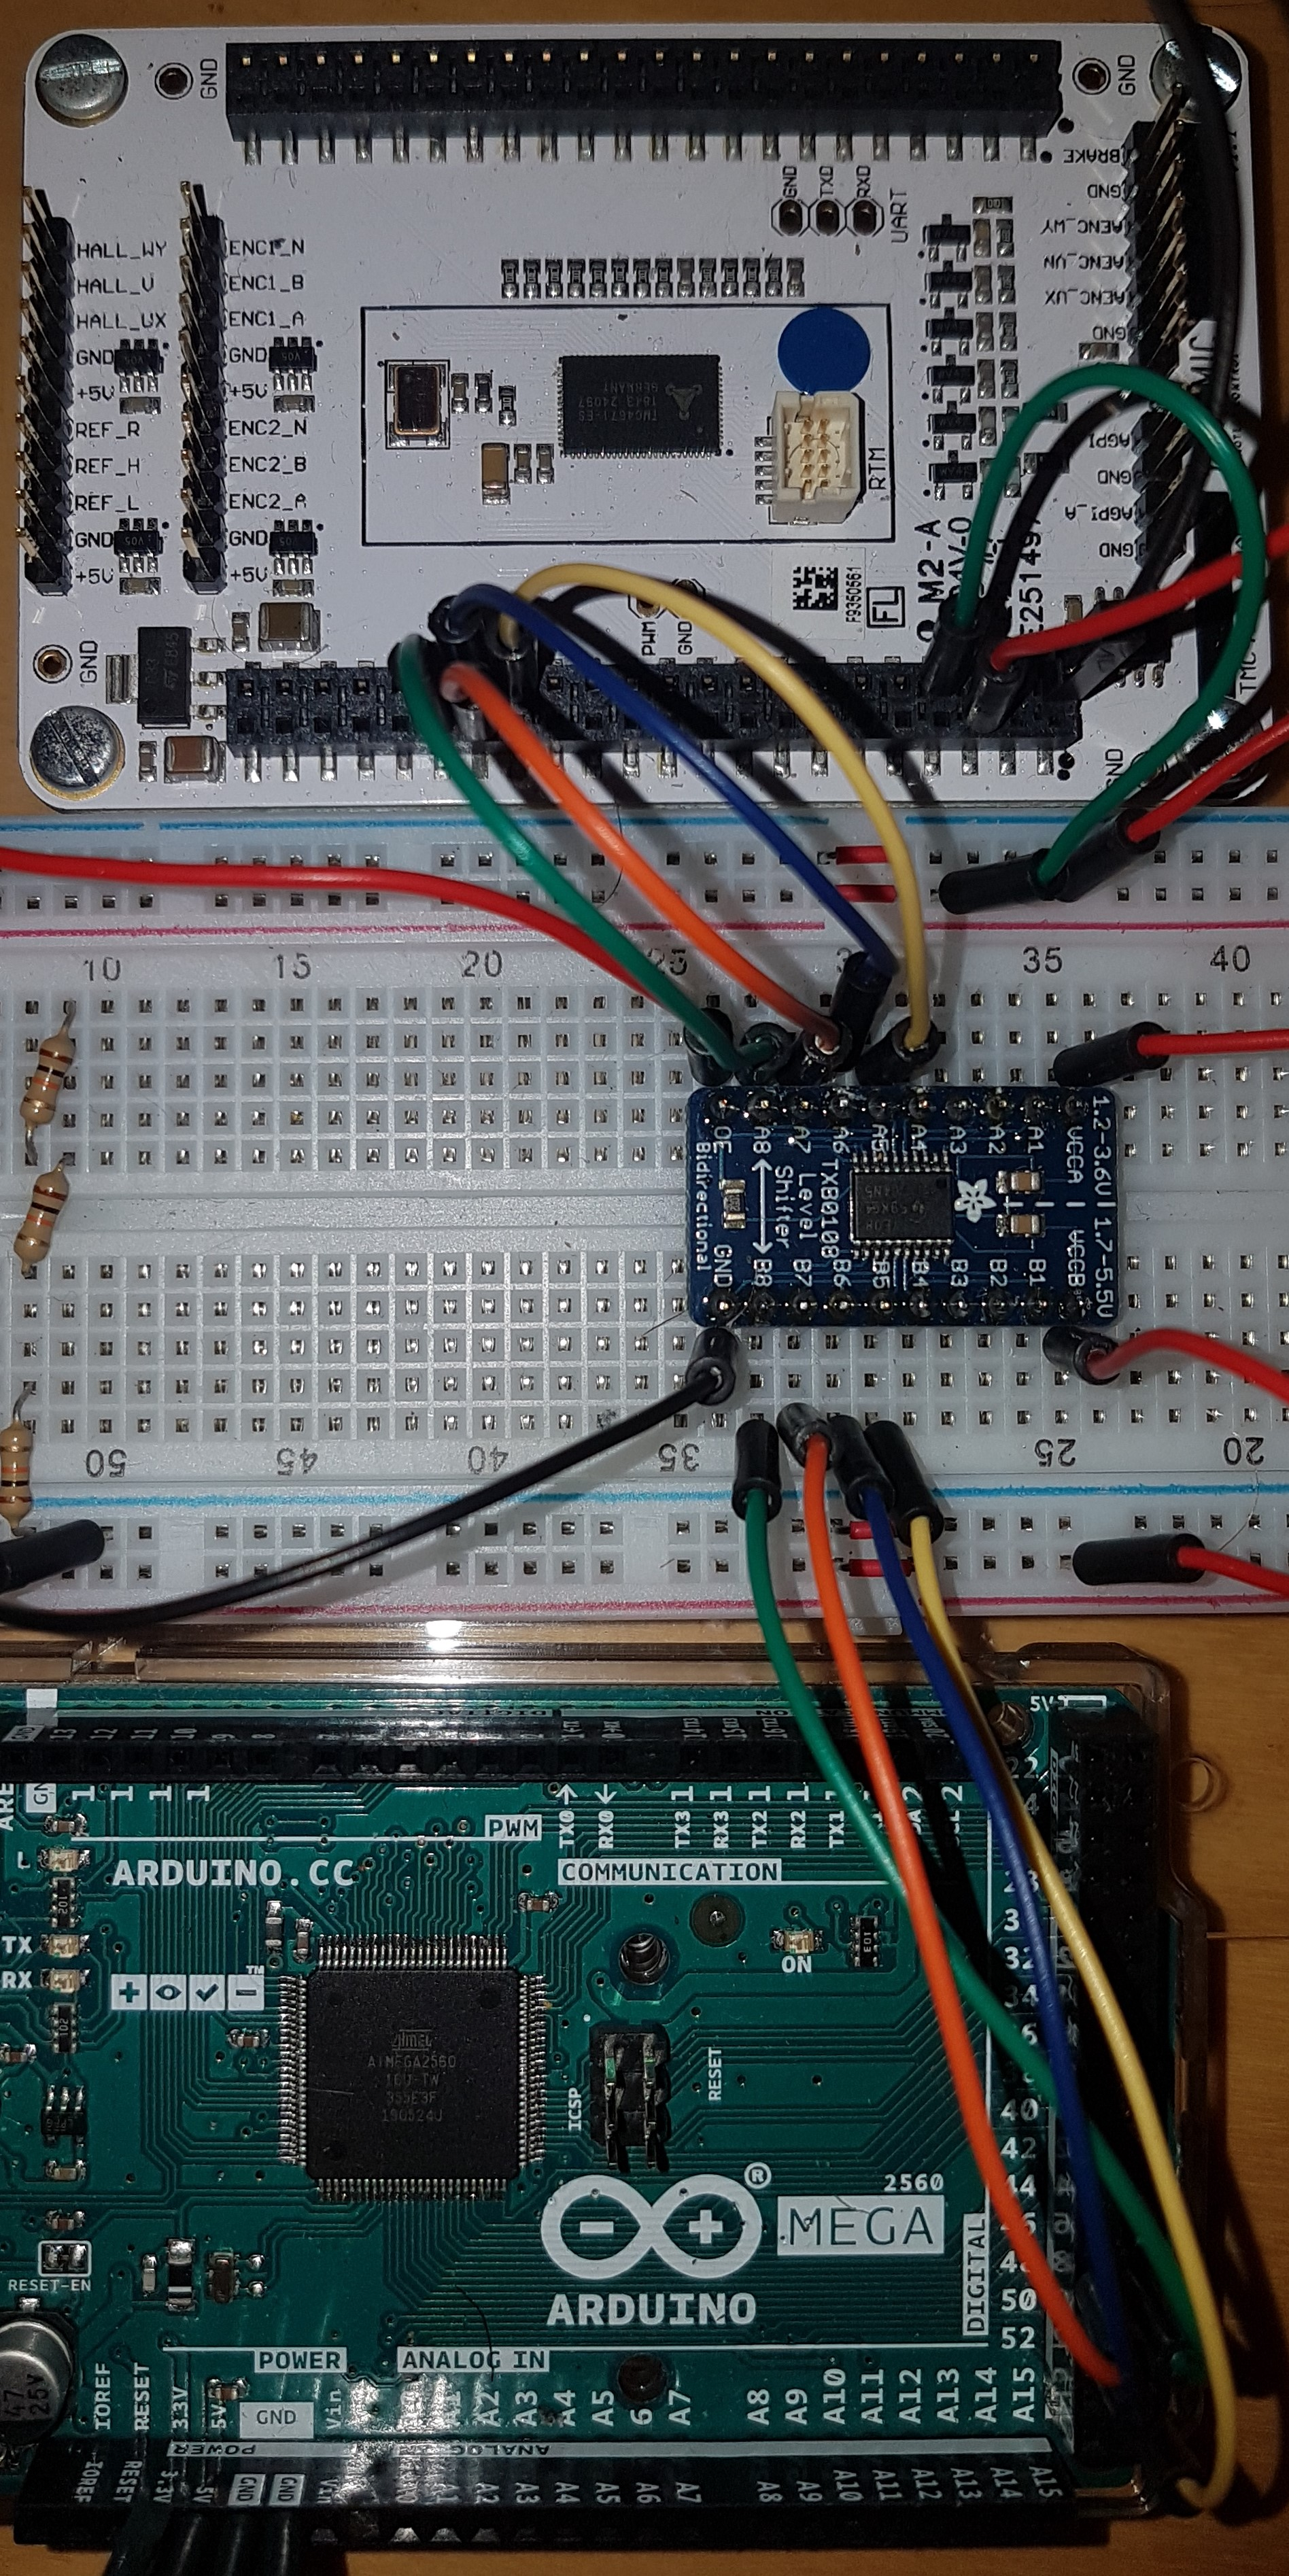
\includegraphics[angle=270,width=0.8 \textwidth]{graphics/1_komplett}
	\caption{Gesamtansicht Setup.}
	\label{fig:1_komplett}
\end{figure}

\textbf{Achtung}, wenn die Scripts auf den Mikrocontroller des PartyMixers geladen werden ist darauf zu achten, dass die Achse des Motors frei beweglich ist und das Förderband nicht mit der Achse mitdreht, da ansonsten Schäden an der Maschine entstehen können. Es wird empfohlen die Scripts mit Mikrocontroller und EVAL-Boards zu testen oder den Motor aus dem Partymixer auszubauen.

Vorgehen:
\begin{enumerate}
\item Benötigte Applikation, welche im Software-Ordner auf dem USB-Stick oder Github \cite{aebi_projekt-6softwareatmega_2020} zu finden ist, in Atmel Studio öffnen.\\
\textcolor{magenta}{Software\textrightarrow Atmega\textrightarrow 3\underline{ }Motor\underline{ }Openloop\textrightarrow 1\underline{ }Motor\underline{ }Testsoftware\textrightarrow Motor}\\

\item Software anpassen: Zeile 23 bis 32\\
\textcolor{OliveGreen}{
	initTMC4671\underline{ }Openloop();\\
\\
    while (1) \\
    \{\\
		\underline{ }delay\underline{ }ms(10000);\\
		read\underline{ }registers\underline{ }TMC4671();\\
    \}
}\\

\item Software hochladen:\\
\textcolor{blue}{AtmelStudio\textrightarrow Tools\textrightarrow PartyMixer}\\
\end{enumerate}

Ergebnis: Nach Hochladen der Software liegen die gewünschten Signale an. Da kein Motor angeschlossen ist, müssen die Signale gemessen werden. Nach dem Testdrive werden im 10 Sekunden-Takt diverse aus dem FOC-Treiber ausgelesene Register ausgegeben.

Im Anhang Kapitel \ref{Appendix:TMC4671_SPI} sind die Messbilder zur SPI- Kommunikation zu finden und in Anhang \ref{Appendix:TMC4671_Gate_Ctrl} die Messbilder zur Gate-Control vom FOC-Treiber zum Gate-Treiber während des Closed-Loops. Beide Signale sind sauber.